% This file was created with tikzplotlib v0.10.1.
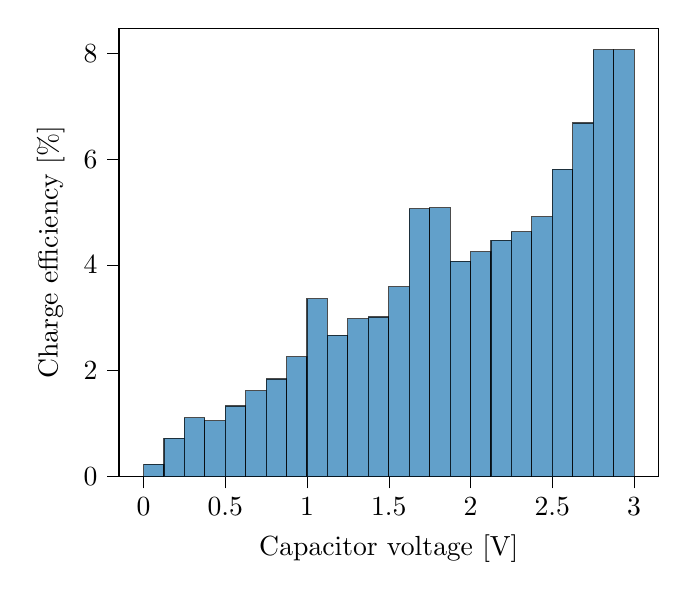
\begin{tikzpicture}

\definecolor{darkgray176}{RGB}{176,176,176}
\definecolor{steelblue31119180}{RGB}{31,119,180}

\begin{axis}[
tick align=outside,
tick pos=left,
x grid style={darkgray176},
xlabel={Capacitor voltage [V]},
xmin=-0.15, xmax=3.15,
xtick style={color=black},
y grid style={darkgray176},
ylabel={Charge efficiency [\%]},
ymin=0, ymax=8.47336960348718,
ytick style={color=black}
]
\draw[draw=black,fill=steelblue31119180,opacity=0.7] (axis cs:0,0) rectangle (axis cs:0.125,0.228423433141316);
\draw[draw=black,fill=steelblue31119180,opacity=0.7] (axis cs:0.125,0) rectangle (axis cs:0.25,0.721730096318468);
\draw[draw=black,fill=steelblue31119180,opacity=0.7] (axis cs:0.25,0) rectangle (axis cs:0.375,1.11142821753546);
\draw[draw=black,fill=steelblue31119180,opacity=0.7] (axis cs:0.375,0) rectangle (axis cs:0.5,1.05515746129777);
\draw[draw=black,fill=steelblue31119180,opacity=0.7] (axis cs:0.5,0) rectangle (axis cs:0.625,1.33346244745136);
\draw[draw=black,fill=steelblue31119180,opacity=0.7] (axis cs:0.625,0) rectangle (axis cs:0.75,1.62631238864569);
\draw[draw=black,fill=steelblue31119180,opacity=0.7] (axis cs:0.75,0) rectangle (axis cs:0.875,1.84414861795885);
\draw[draw=black,fill=steelblue31119180,opacity=0.7] (axis cs:0.875,0) rectangle (axis cs:1,2.26789085503476);
\draw[draw=black,fill=steelblue31119180,opacity=0.7] (axis cs:1,0) rectangle (axis cs:1.125,3.36186177981046);
\draw[draw=black,fill=steelblue31119180,opacity=0.7] (axis cs:1.125,0) rectangle (axis cs:1.25,2.67291889666291);
\draw[draw=black,fill=steelblue31119180,opacity=0.7] (axis cs:1.25,0) rectangle (axis cs:1.375,2.98569711638251);
\draw[draw=black,fill=steelblue31119180,opacity=0.7] (axis cs:1.375,0) rectangle (axis cs:1.5,3.01509836141522);
\draw[draw=black,fill=steelblue31119180,opacity=0.7] (axis cs:1.5,0) rectangle (axis cs:1.625,3.58910158924856);
\draw[draw=black,fill=steelblue31119180,opacity=0.7] (axis cs:1.625,0) rectangle (axis cs:1.75,5.06402456856152);
\draw[draw=black,fill=steelblue31119180,opacity=0.7] (axis cs:1.75,0) rectangle (axis cs:1.875,5.07859353056663);
\draw[draw=black,fill=steelblue31119180,opacity=0.7] (axis cs:1.875,0) rectangle (axis cs:2,4.07223810086736);
\draw[draw=black,fill=steelblue31119180,opacity=0.7] (axis cs:2,0) rectangle (axis cs:2.125,4.24718421881433);
\draw[draw=black,fill=steelblue31119180,opacity=0.7] (axis cs:2.125,0) rectangle (axis cs:2.25,4.4667288277064);
\draw[draw=black,fill=steelblue31119180,opacity=0.7] (axis cs:2.25,0) rectangle (axis cs:2.375,4.62959438856094);
\draw[draw=black,fill=steelblue31119180,opacity=0.7] (axis cs:2.375,0) rectangle (axis cs:2.5,4.91471042483022);
\draw[draw=black,fill=steelblue31119180,opacity=0.7] (axis cs:2.5,0) rectangle (axis cs:2.625,5.80725563608463);
\draw[draw=black,fill=steelblue31119180,opacity=0.7] (axis cs:2.625,0) rectangle (axis cs:2.75,6.68152973021969);
\draw[draw=black,fill=steelblue31119180,opacity=0.7] (axis cs:2.75,0) rectangle (axis cs:2.875,8.0696054701819);
\draw[draw=black,fill=steelblue31119180,opacity=0.7] (axis cs:2.875,0) rectangle (axis cs:3,8.06987581284493);
\end{axis}

\end{tikzpicture}
